\documentclass{cumcm}
\usepackage{graphicx}
\usepackage{appendix}
\numberwithin{equation}{section}
\numberwithin{equation}{subsection}
\usepackage{csvsimple}
\usepackage{listings}
\usepackage{xcolor}
%\renewcommand{\baselinestretch}{1.0}
%\newcommand{\songtiB}

% \title{text}这里是显示在第三页的文章标题
\title{\textbf{计算机系统结构实验报告\quad 实验2}\\{\Large FPGA基础实验: 4-bit Adder}}
\author{方泓杰\ 518030910150}


\begin{document}
\maketitle

\begin{abstract}
  本实验实现了FPGA基础实验中的四位全加器。该器件支持带进位的$4$位二进制数的加法,输入两个$4$位二进制数,输出一个$4$位二进制数表示输入的两个数相加的结果,并且支持接收上一部分的进位结果与传递下一部分的进位结果。我们通过与、或、异或等简单的逻辑运算实现一位全加器,并通过其来进一步实现四位全加器。本实验通过软件仿真的形式进行实验结果的验证。
\end{abstract}

\maketitle \tableofcontents
\newpage

\section{实验目的}\label{section1}
本次实验有如下四个实验目的:
\begin{enumerate}
    \item 熟悉Xilinx逻辑设计工具Vivado的基本操作;
    \item 掌握使用VerilogHDL进行简单的逻辑设计;
    \item 理解一位全加器与四位全加器的工作原理;
    \item 使用功能仿真验证功能实现的正确性。
\end{enumerate}

\section{原理分析}\label{section2}
\subsection{一位全加器原理分析}\label{section2.1}
一位全加器包括$a$,$b$和$c_i$三个1位输入端,分别表示输入的两个数与接收到的上一部分的进位结果;包括$s$和$c_o$两个1位输出端,分别表示加法运算结果与需要传递到下一部分的进位结果。其真值表如下:

\begin{table}[htbp]
    \centering
    \begin{tabular}{|ccc|cc|}
         \hline
         $a$ & $b$ & $c_i$ & $s$ & $c_o$\\
         \hline
         0 & 0 & 0 & 0 & 0 \\
         0 & 0 & 1 & 1 & 0 \\
         0 & 1 & 0 & 1 & 0 \\
         0 & 1 & 1 & 0 & 1 \\
         1 & 0 & 0 & 1 & 0 \\
         1 & 0 & 1 & 0 & 1 \\
         1 & 1 & 0 & 0 & 1 \\
         1 & 1 & 1 & 1 & 1 \\
         \hline
    \end{tabular}
    \caption{一位全加器的真值表}
    \label{tab1}
\end{table}

一位全加器的原理较为简单,即实现能表达上述真值表(表 \ref{tab1})的逻辑电路即可。分析真值表后可以发现输出端与输入端的逻辑关系如下:

\begin{equation}\label{eq1}
\begin{aligned}
s &= a \oplus b \oplus c_i \\
c_o &= (a \land b) \lor (a \land c_i) \lor (b \land c_i)
\end{aligned}
\end{equation}

其中,$\oplus$ 表示逻辑异或。

\subsection{四位全加器原理分析}\label{section2.2}
四位全加器包括$a$,$b$两个4位输入端和$c_i$一个1位输入端,分别表示输入的两个数与接收到的上一部分的进位结果;包括$s$一个4位输出端和$c_o$一个1位输出端,分别表示加法运算结果与需要传递到下一部分的进位结果。

四位全加器可以看成四个一位全加器串联组成,前一个一位全加器的$c_o$端接入后一个一位全加器的$c_i$端,第一个一位全加器的$c_i$端为整个四位全加器的$c_i$端,最后一个一位全加器的$c_o$端为整个四位全加器的$c_o$端。同时,我们将四位全加器的两个4位输入$a$与$b$分成四个对应部分,分别分配给每一个一位全加器进行运算,并且把四个一位全加器运算结果合并,得到最终的四位全加器的输出$s$。其电路逻辑示意图如图 \ref{fig1} 所示。

\begin{figure}[htbp]
    \centering
    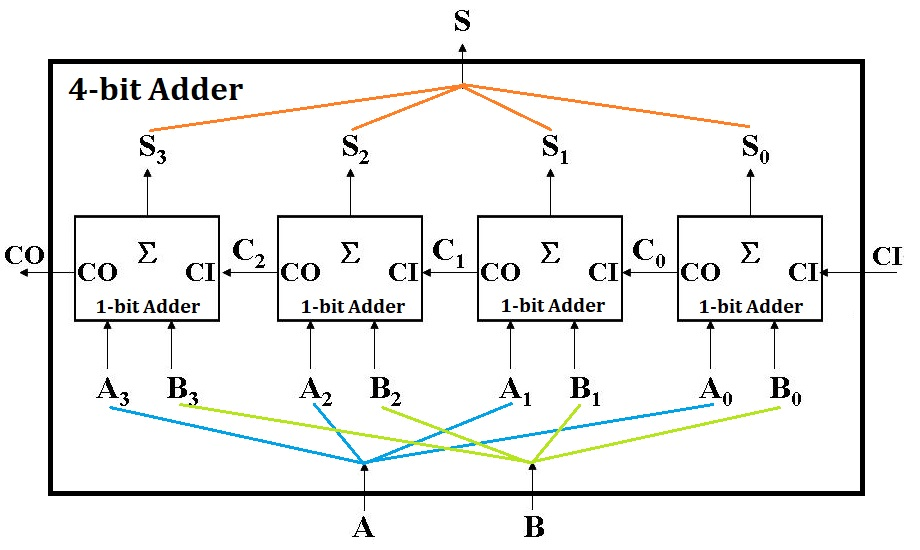
\includegraphics[width=6in]{4bit-adder.jpg}
    \caption{四位全加器的电路逻辑示意图}
    \label{fig1}
\end{figure}

\section{功能实现}\label{section3}

\subsection{一位全加器的功能实现}\label{section3.1}

根据 \ref{section2.1} 节中式 \eqref{eq1} 所展示的输出端逻辑表达式,我们可以设计代码进行实现;由于逻辑表达式较为复杂,我们需要设计$s_1,c_1,c_2,c_3$这四个中间变量存储运算的中间结果。具体代码实现如下所示;注意这里的 \texttt{and}, \texttt{or} 和 \texttt{xor} 均为Verilog自带的逻辑运算单元,可以直接使用。

\begin{lstlisting}[language=verilog]
wire s1, c1, c2, c3;
and (c1, a, b),
    (c2, b, ci),
    (c3, a, ci);
xor (s1, a, b),
    (s, s1, ci);
or (co, c1, c2, c3);
\end{lstlisting}

完整的代码实现参见附录 \ref{appsection1.1}。

\subsection{四位全加器的功能实现}\label{section3.2}

根据 \ref{section2.2} 节中图 \ref{fig1} 所示的四位全加器的电路逻辑示意图,我们可以利用四个一位全加器串联实现四位全加器的功能。前一个一位全加器的$c_o$端接入后一个一位全加器的$c_i$端,第一个一位全加器的$c_i$端为整个四位全加器的$c_i$端,最后一个一位全加器的$c_o$端为整个四位全加器的$c_o$端。同时,我们设置三个中间变量$ct_0, ct_1, ct_2$存储进位的中间结果。具体代码实现如下所示:
\begin{lstlisting}[language=verilog]
wire [2 : 0] ct;
adder_1bit a1(.a(a[0]), .b(b[0]), .ci(ci), .s(s[0]), .co(ct[0])),
           a2(.a(a[1]), .b(b[1]), .ci(ct[0]), .s(s[1]), .co(ct[1])),
           a3(.a(a[2]), .b(b[2]), .ci(ct[1]), .s(s[2]), .co(ct[2])),
           a4(.a(a[3]), .b(b[3]), .ci(ct[2]), .s(s[3]), .co(co));
\end{lstlisting}

完整的代码实现参见附录 \ref{appsection1.2}。

\section{结果验证}\label{section4}
我们使用Verilog编写激励文件,采用软件仿真的形式对四位全加器进行测试(代码实现参见附录 \ref{appsection2})。我们在激励文件中使用了多组不同的数据进行测试,测试结果如图 \ref{fig2} 所示。

\begin{figure}[htbp]
    \centering
    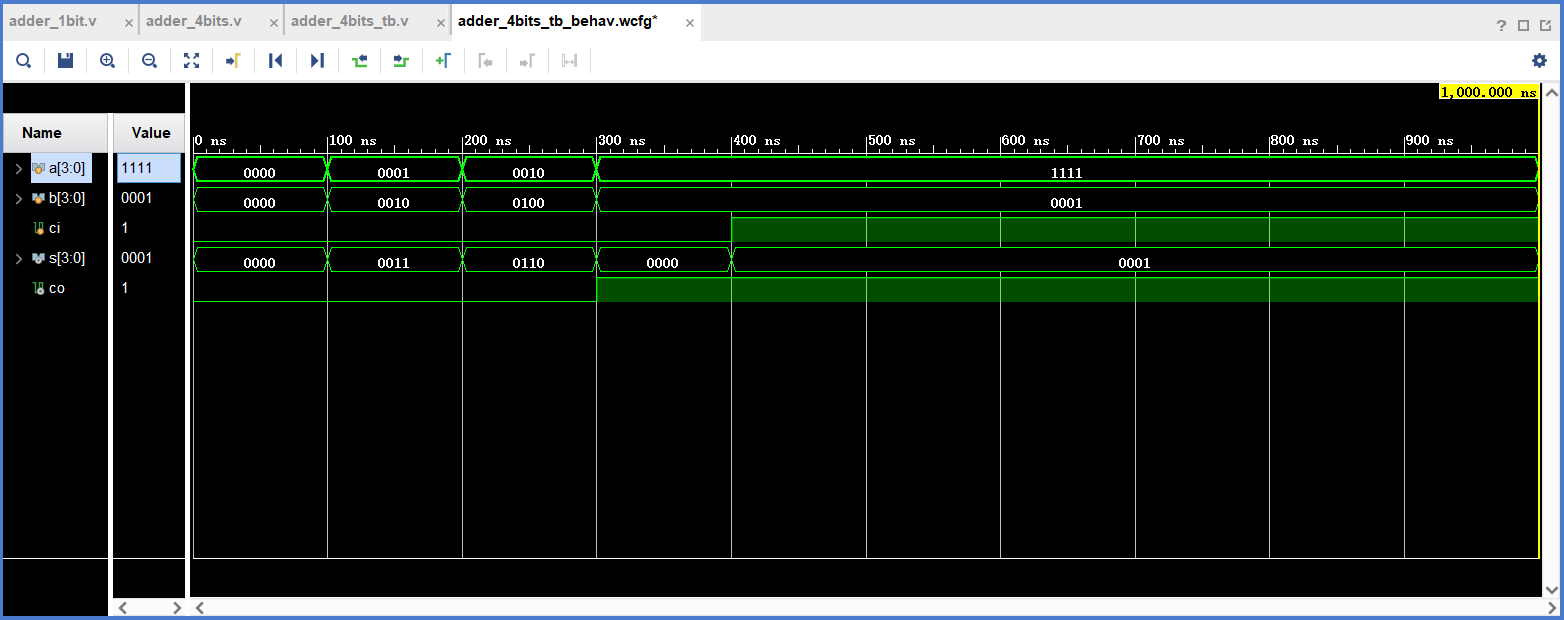
\includegraphics[width=6.3in]{1.png}
    \caption{四位全加器的测试结果}
    \label{fig2}
\end{figure}

从图 \ref{fig2} 中可以看出,我们完成了四位全加器的功能实现,并且仿真结果正确。

\section{总结与反思}\label{section5}

本实验实现了FPGA实验中四位全加器这一基础部件的设计与仿真。实现这一部件的主要方法是化繁为简,首先实现基础的一位全加器,再将其进行组合连接得到最终的四位全加器。对于一位全加器的实现,我们首先列写出其真值表,然后通过真值表找规律以及逻辑推理等方法,推导出输出与输入的逻辑表达式,然后利用Verilog自带的与、或以及异或元件进行操作。通过这次试验,我对于Xillinx逻辑设计工具Vivado有了一些较为深入的认识,已经可以熟练运用Verilog语言进行基础的逻辑设计以及基础的仿真模拟,为后面几次实验的复杂逻辑设计与仿真奠定了基础。

实验中利用了“子元件”的思想我认为非常重要,这种思想可以将一个较为复杂的元件拆分成许多功能简单、易于实现的元件,最后进行组装连接。这种思想在接下来的单周期MIPS设计实验以及最后的流水线设计实验中都有着广泛的应用。

除四位全加器以外,我认为我们也可以利用类似的方法实现更加复杂的器件,如32位加法器以及乘法器等等,熟练掌握这种方法令我受益匪浅。

\section{致谢}\label{section6}
感谢本次实验中指导老师在课程微信群里为同学们答疑解惑;

感谢上海交通大学网络信息中心提供的远程桌面资源;

感谢计算机科学与工程系相关老师对于课程指导书的编写以及对于课程的设计,让我们可以更快更好地学习相关知识,掌握相关技能;

感谢电子信息与电气工程学院提供的优秀的课程资源。
%\bibliographystyle{plain}
%\bibliography{ref}

\clearpage
\begin{appendices}
\section{设计文件完整代码实现}\label{appsection1}
\subsection{一位全加器的代码实现}\label{appsection1.1}
参见代码文件 \texttt{adder\_1bit.v}。
\subsection{四位全加器的代码实现}\label{appsection1.2}
参见代码文件 \texttt{adder\_4bits.v}。
\section{激励文件完整代码实现}\label{appsection2}
参见代码文件 \texttt{adder\_4bits\_tb.v}。
\end{appendices}

\end{document}
